%%%%%%%%%%%%%%%%%%%%%%%%%%%%%%%%%%%%%%%%%
% University/School Laboratory Report
% LaTeX Template
% Version 3.1 (25/3/14)
%
% This template has been downloaded from:
% http://www.LaTeXTemplates.com
%
% Original author:
% Linux and Unix Users Group at Virginia Tech Wiki 
% (https://vtluug.org/wiki/Example_LaTeX_chem_lab_report)
%
% License:
% CC BY-NC-SA 3.0 (http://creativecommons.org/licenses/by-nc-sa/3.0/)
%
%%%%%%%%%%%%%%%%%%%%%%%%%%%%%%%%%%%%%%%%%

%----------------------------------------------------------------------------------------
%	PACKAGES AND DOCUMENT CONFIGURATIONS
%----------------------------------------------------------------------------------------

\documentclass{article}

\usepackage{array}
\usepackage{tabularx}
\usepackage{geometry}
\usepackage{graphicx} % Required for the inclusion of images
\usepackage[utf8]{inputenc}
\usepackage[english]{babel}
\usepackage{minted}
\usemintedstyle{borland}
\usepackage{xcolor}
\setlength\parindent{1.2pt} % Removes all indentation from paragraphs

\renewcommand{\labelenumi}{\alph{enumi}.} % Make numbering in the enumerate environment by letter rather than number (e.g. subsection 6)
\geometry{
 a4paper,
 total={170mm,257mm},
 left=20mm,
 top=20mm,
 }
%\usepackage{times} % Uncomment to use the Times New Roman font

%----------------------------------------------------------------------------------------
%	DOCUMENT INFORMATION
%----------------------------------------------------------------------------------------

\title{
	Microcontroller Lab Report \\
\large 8086 programming Part 2b
} % Title

\author{
	Aaditya Prakash Kattekola \\
	{\small Roll: 194201} \\
	{\small ECE Section B} \\
} % Author name

\date{August 28, 2021} % Date for the report

\begin{document}

\maketitle % Insert the title, author and date

% If you wish to include an abstract, uncomment the lines below
% \begin{abstract}
% Abstract text
% \end{abstract}

%----------------------------------------------------------------------------------------
%	Question 1
%----------------------------------------------------------------------------------------

\break
\section{Question 1}
%----------------------------------------------------------------------------------------
%	subsection 1
%----------------------------------------------------------------------------------------

\subsection{Aim}
Write the assembly language program for 8086 MP to find the sum of absolute difference between two arrays. Array are available in a connected memory. Length of the array is N. Where N represent the last 2 digits of your roll number. 
(Since array of length 01 is not ideal, I used array of length 5)
%----------------------------------------------------------------------------------------
%	subsection 2
%----------------------------------------------------------------------------------------

\subsection{Program}
\subsubsection{Code}
\inputminted{nasm}{"C:/Users/aadit/Documents/BTech/5th Semester/MC Lab/8086 Pgrm 2/2B/SAD.asm"}

\subsubsection{Emulator}

\begin{center}
\begin{tabularx}{1.0\textwidth} { 
  | >{\centering\arraybackslash}X 
  | >{\centering\arraybackslash}X 
  | >{\centering\arraybackslash}X | }
 \hline
\textbf{Address  (CS:0100, IP:0000)} &\textbf{Machine code}&\textbf{Instruction} \\
  \hline
 01000 & B1, 05 & MOV CL, 05H \\ 
  \hline
  01002 & BE, 00, C9 & MOV SI, 0C900H \\
  \hline
 01005 & BA, 00, 00 & 00000H \\
 \hline
 01008 & 8A, 04 & MOV AL, [SI] \\
 \hline
 0100A & 8A, 5C, 05 & MOV BL, [SI] + 05H \\
 \hline
 0100D & 2B, C3 & SUB AX, BX \\
 \hline
 0100F & 79, 02 & JNS 013H \\
 \hline
 01011 & F7, D8 & NEG AX \\
 \hline
 01013 & 02, D0 & ADD DL, AL \\
 \hline
 01015 & 46 & INC SI \\
 \hline
 01016 & FE, C9 & DEC CL \\
 \hline
 01018 & 75, EE & JNE 08H \\
 \hline
 0101A & F4 & HLT \\  
  \hline
\end{tabularx}
\end{center}

%----------------------------------------------------------------------------------------
%	subsection 3
%----------------------------------------------------------------------------------------
\break
\subsection{Result}
\subsubsection{Input}
\begin{figure}[h]
\begin{center}
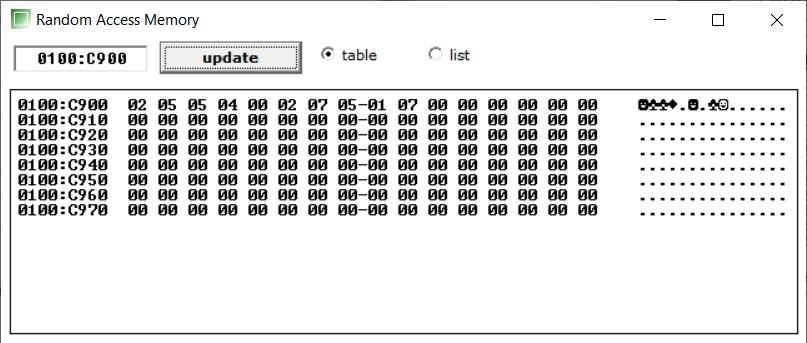
\includegraphics[width=0.8\textwidth]{SAD_IN} 
\caption{RAM Input for Q1}
\end{center}
\end{figure}

\subsubsection{Expectation}
$ SI \leftarrow C900H \\
AX \leftarrow 
\ |\ \lbrack SI  \rbrack - \lbrack SI - 1 \rbrack\  |\\
DX \leftarrow DX + AX  \\
Final\ Ans:\  C\ (12\ in\ DEC)\ in\ DX \\ 
$ 

%----------------------------------------------------------------------------------------
%	subsection 4
%----------------------------------------------------------------------------------------
\break
\subsubsection{Emulator}

\begin{figure}[h]
\begin{center}
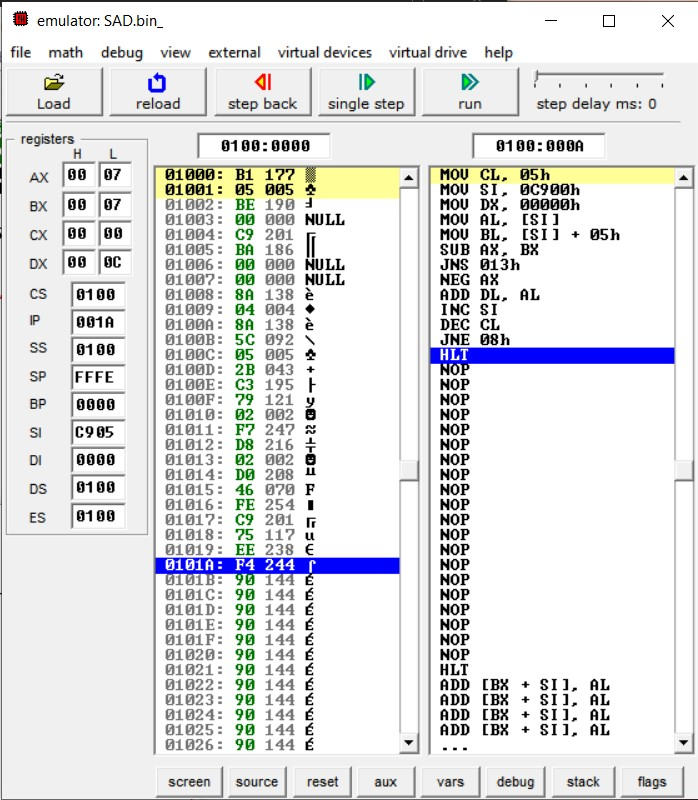
\includegraphics[width=0.75\textwidth]{SAD_OUT} 
\caption{STACK Output for Q1}
\end{center}
\end{figure}


%----------------------------------------------------------------------------------------
%	Question 2
%----------------------------------------------------------------------------------------

\break
\section{Question 2}
%----------------------------------------------------------------------------------------
%	subsection 1
%----------------------------------------------------------------------------------------

\subsection{Aim}
Write an assembly language program for 8086 MP to model the 4x16 decoder.
%----------------------------------------------------------------------------------------
%	subsection 2
%----------------------------------------------------------------------------------------

\subsection{Program}
\subsubsection{Code}
\inputminted{nasm}{"C:/Users/aadit/Documents/BTech/5th Semester/MC Lab/8086 Pgrm 2/2B/4X16.asm"}

\subsubsection{Emulator}

\begin{center}
\begin{tabularx}{1.0\textwidth} { 
  | >{\centering\arraybackslash}X 
  | >{\centering\arraybackslash}X 
  | >{\centering\arraybackslash}X | }
 \hline
\textbf{Address  (CS:0100, IP:0000)} &\textbf{Machine code}&\textbf{Instruction} \\
  \hline
 01000 & B1, 09 & MOV CL, 09H \\ 
  \hline
 01002 & BA, 00, 80 & MOV DX, 08000H \\
 \hline
 01005 & D3, EA & SHR DX, CL \\
 \hline
 01007 & F4 & HLT \\  
  \hline
\end{tabularx}
\end{center}

%----------------------------------------------------------------------------------------
%	subsection 3
%----------------------------------------------------------------------------------------
\break
\subsection{Result}
\subsubsection{Input}
 CL: 1001B ; $s_3 s_2 s_1 s_0 $ \\
 DX:\ 1000\ 0000\ 0000\ 0000\ (8000\ in HEX)
 
\subsubsection{Expectation}
$
DX \leftarrow DX \gg CL \\
8000H \gg 09H \rightarrow 0040H\ in\ DX 
$ 

%----------------------------------------------------------------------------------------
%	subsection 4
%----------------------------------------------------------------------------------------

\subsubsection{Emulator}
\begin{figure}[h]
\begin{center}
\includegraphics[width=0.65\textwidth]{4x16_OUT} 
\caption{STACK Output for Q2}
\end{center}
\end{figure}

\end{document}